\chapter{البلورات \texorpdfstring{\babelsublr{(1)}}{(1)}: البلورة المثالية والفلزات}\label{ch:b1:crystals-metals}

يمكن سحب سلك من النحاس حتى يصير أرق من شعرة دون أن ينقطع؛ أما كتلة
الملح فتتحطم تحت المطرقة. ويسخّن الحداد قضيبًا من الحديد حتى
يتوهج، ويطرقه، ويغمسه في الماء، فيخرج القضيب أشد صلادة بكثير مما
دخل. والفرق بين هذه السلوكات كامن في طريقة تراصّ الذرات
في الجسم الصلب. فأكثر الأجسام الصلبة بلورات: ذراتها مرتبة وفق نمط يتكرر
بعينه مليارات المرات في كل اتجاه. يصف هذا الفصل هذه الأنماط، ويعدّ
ذراتها، ويقيس مدى تراصّها وأين تقع الفجوات
بينها، ويستعمل النتيجة لفهم الفلزات والسبائك.
ويطبّق الفصل التالي الأدوات نفسها على الأجسام الصلبة الأيونية والتساهمية
والجزيئية.

\begin{recall}
تفقد الفلزات إلكترونات تكافئها بسهولة: فطاقات تأينها
وكهرسلبياتها منخفضة (\cref{ch:b1:periodicity}). وقد عُرّفت أنصاف الأقطار الذرية
في \cref{def:b1:periodicity:radius}. وتُستعمل الكتلة الحجمية، وهي خاصية
تدرسها الفيزياء، على أنها معلومة: $\rho = m/V$.
\end{recall}

\begin{omfigure}
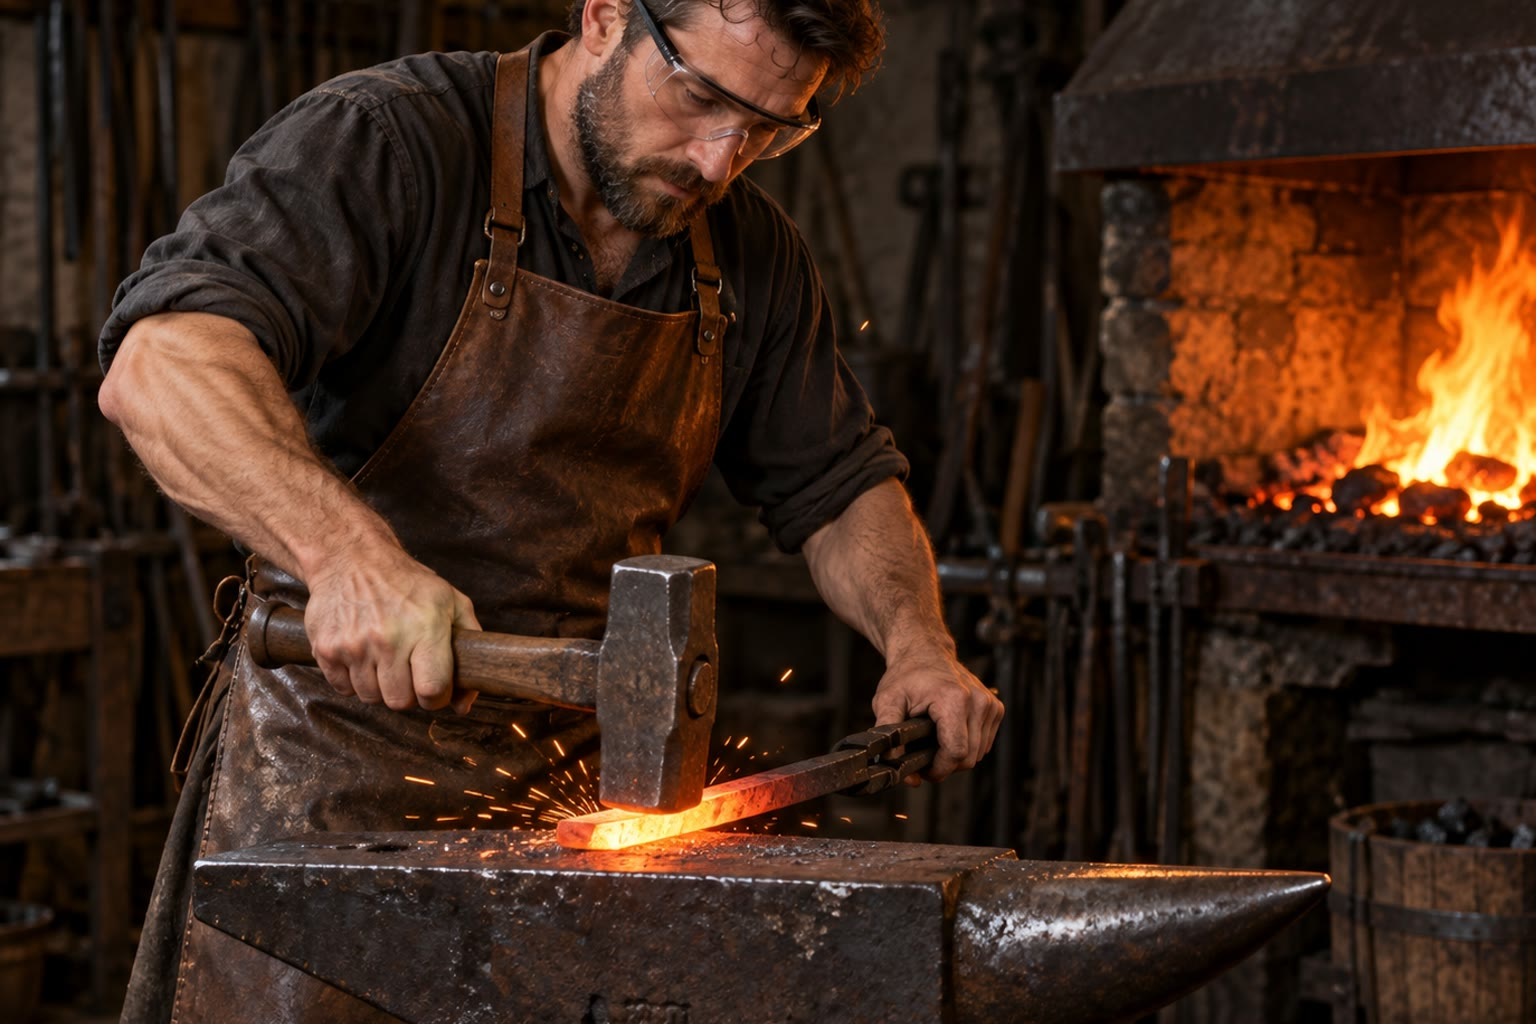
\includegraphics[width=0.55\linewidth]{images/book2/ai/b1-05-blacksmith.jpg}

{\small حداد يطرق الفولاذ. للحديد المتوهج بالبرتقالي
بنية بلورية تختلف عن بنية الحديد في درجة حرارة الغرفة، ويستطيع أن يحوي
كربونًا أكثر (مسألة نهاية الأسبوع).}
\end{omfigure}

\section{نموذج البلورة المثالية}

\begin{definition}[البلورة، الجسم الصلب اللابلوري، البلورة المثالية]\label{def:b1:crystals-metals:crystal}
\emph{البلورة}\index{بلورة} جسم صلب جسيماته (ذرات أو أيونات
أو جزيئات) مرتبة وفق نمط يتكرر دوريًا في
الأبعاد الثلاثة. والجسم الصلب الخالي من هذا الترتيب البعيد المدى
\emph{جسم صلب لابلوري}\index{جسم صلب لابلوري} (الزجاج، وأكثر اللدائن).
و\emph{نموذج البلورة المثالية}\index{نموذج البلورة المثالية} يصف
البلورة لانهائية وخالية من العيوب: لا ذرات ناقصة ولا زائدة، ولا
شوائب، ولا حدود.
\end{definition}

\begin{definition}[الشبكة، النقش، الخلية الأولية]\label{def:b1:crystals-metals:lattice}
\emph{الشبكة}\index{شبكة} مجموعة لانهائية من النقاط، هي
\emph{العقد}\index{عقدة}، تُستخرج من إحداها بكل
الانسحابات $u\,\vec a + v\,\vec b + w\,\vec c$ حيث $u$ و$v$
و$w$ أعداد صحيحة. وتُستخرج \omterm{def:b1:crystals-metals:crystal}{البلورة} بوضع
\emph{النقش}\index{نقش} نفسه على كل عقدة (ذرة واحدة، أو مجموعة ذرات أو أيونات).
و\emph{الخلية الأولية}\index{خلية أولية} متوازي سطوح مبني على
$\vec a$ و$\vec b$ و$\vec c$ تملأ انسحاباته الفضاء؛ وأطوال أحرفه
وزواياه هي \emph{وسائط الشبكة}\index{وسائط الشبكة}
$a$، $b$، $c$، $\alpha$، $\beta$، $\gamma$. وفي الخلية المكعبة
$a = b = c$ والزوايا $90^\circ$.
\end{definition}

\begin{remark}[البلورات الحقيقية]\label{rem:b1:crystals-metals:real}
البلورات الحقيقية محدودة وغير مثالية: فيها فجوات شاغرة،
وشوائب، وانخلاعات، وحدود حبيبات، تتحكم في كثير من
الخواص (مطيلية النحاس، وصلادة الفولاذ). وتُدرس هذه
العيوب في مجلد السنة الثالثة؛ أما \omterm{def:b1:crystals-metals:crystal}{البلورة} المثالية فتعطي
الهندسة والكتلة الحجمية \omterm{def:b1:crystals-metals:compactness}{والاكتناز}، التي تكاد العيوب لا تغيّرها.
\end{remark}

\begin{definition}[تعددية الخلية]\label{def:b1:crystals-metals:multiplicity}
\emph{التعددية}\index{تعددية} $Z$ لخلية هي عدد
النقوش (أو الذرات) التي تعود إليها، وكل ذرة مشتركة مع
الخلايا المجاورة تُحسب بالكسر الواقع منها داخل الخلية.
\end{definition}

\begin{method}[عدّ ذرات خلية]\label{met:b1:crystals-metals:count}
في الخلية المكعبة تشترك في الذرة الواقعة على رأس 8 خلايا فتُحسب
$1/8$؛ وعلى حرف تشترك فيها 4 فتُحسب $1/4$؛ وعلى وجه
تشترك فيها 2 فتُحسب $1/2$؛ وفي الداخل تُحسب 1. ثم اجمع الإسهامات.
\end{method}

\begin{definition}[عدد التناسق]\label{def:b1:crystals-metals:coordination}
\emph{عدد التناسق}\index{عدد التناسق} لجسيم
في جسم صلب هو عدد أقرب جيرانه، أي الواقعين على
أقصر مسافة.
\end{definition}

\begin{definition}[الاكتناز]\label{def:b1:crystals-metals:compactness}
\emph{الاكتناز}\index{اكتناز} (أو معامل الملء) في
\omterm{def:b1:crystals-metals:crystal}{بلورة} من كرات صلبة هو كسر الحجم الذي تشغله
الكرات: من أجل خلية حجمها $V$ تحوي $Z$ كرة نصف قطرها $R$،
\[
  C = \frac{Z \cdot \frac43 \pi R^3}{V} .
\]
\end{definition}

\begin{proposition}[الكتلة الحجمية انطلاقًا من الخلية]\label{prop:b1:crystals-metals:density}
الكتلة الحجمية \omterm{def:b1:crystals-metals:crystal}{لبلورة} تحوي خليتها، التي حجمها $V$، عدد $Z$ من
الجسيمات كتلتها المولية $M$ هي
\[
  \rho = \frac{Z\,M}{N_A\,V} .
\]
\end{proposition}

\begin{proof}
تحوي الخلية $Z$ جسيمًا، كتلتها $Z\,M/N_A$؛ \omterm{def:b1:crystals-metals:crystal}{والبلورة} هي
الخلية مكررة، فكتلتها الحجمية هي كتلة خلية واحدة الحجمية.
\end{proof}

\section{الرصّ المتراصّ: المكعب الممركز الأوجه والسداسي}

\begin{definition}[الرصّ المتراصّ، المكعب الممركز الأوجه، السداسي المتراصّ]\label{def:b1:crystals-metals:packings}
يُبنى \emph{الرصّ المتراصّ}\index{رص متراص} لكرات متماثلة
من طبقات متراصّة، تمسّ فيها كل كرة ست كرات أخرى، مكدّسة
بحيث تستقر كل كرة من طبقة في تجويف من الطبقة التي تحتها. فيعطي
التكديس $ABCABC\dots$ بنية \emph{المكعب الممركز الأوجه}\index{مكعب ممركز الأوجه}
(أو المكعب المتراصّ)؛ ويعطي التكديس $ABAB\dots$
بنية \emph{السداسي المتراصّ}\index{سداسي متراص}.
وثمة بنية ثالثة للفلزات غير متراصّة هي بنية
\emph{المكعب الممركز الجسم}\index{مكعب ممركز الجسم}، أي
مكعب بذرة على كل رأس وذرة في مركزه.
\end{definition}

\begin{omfigure}
\begin{tikzpicture}[font=\small]
  % layer A
  \foreach \i in {0,...,4} \foreach \j in {0,...,3} {
    \pgfmathsetmacro\x{\i+0.5*\j}
    \pgfmathsetmacro\y{0.866*\j}
    \draw[black!60, fill=omDef!25] (\x,\y) circle (0.5);
  }
  % layer B, in the hollows pointing up
  \foreach \i/\j in {1/0, 2/0, 3/0, 1/1, 2/1, 3/1, 1/2, 2/2} {
    \pgfmathsetmacro\x{\i+0.5*\j}
    \pgfmathsetmacro\y{0.866*\j+0.577}
    \draw[omThm!80!black, fill=omThm!25, fill opacity=0.75] (\x,\y) circle (0.5);
  }
  % C positions
  \foreach \i/\j in {1/0, 2/0, 3/0, 1/1, 2/1, 3/1} {
    \pgfmathsetmacro\x{\i+0.5+0.5*\j}
    \pgfmathsetmacro\y{0.866*\j+0.289}
    \fill[omMeth] (\x,\y) circle (0.11);
  }
  \node[anchor=west, align=left] at (6.6,1.6) {\foreignlanguage{arabic}{\babelsublr{A}: الطبقة الأولى، بالأزرق}\\\foreignlanguage{arabic}{\babelsublr{B}: الطبقة الثانية، في تجاويف \babelsublr{A}، بالأحمر}\\\foreignlanguage{arabic}{\babelsublr{C}: التجاويف الأخرى، نقاط خضراء}};
\end{tikzpicture}

{\small طبقتان متراصّتان مرئيتان من الأعلى. يمكن لطبقة ثالثة أن تستقر
فوق التجاويف المعلَّمة C (التكديس $ABC$، \omterm{def:b1:crystals-metals:packings}{المكعب الممركز الأوجه}) أو فوق
ذرات A (التكديس $AB$، \omterm{def:b1:crystals-metals:packings}{السداسي المتراصّ}).}
\end{omfigure}

\begin{proposition}[المكعب الممركز الأوجه]\label{prop:b1:crystals-metals:fcc}
في بنية \omterm{def:b1:crystals-metals:packings}{المكعب الممركز الأوجه} تشغل الذرات رؤوس المكعب الثمانية ومراكز
أوجهه الستة، وطول حرفه $a$. فيكون $Z = 4$، \omterm{def:b1:crystals-metals:coordination}{وعدد التناسق}
12، وتتماس الذرات على امتداد قطر الوجه، $a\sqrt2 = 4R$، ويكون
\omterm{def:b1:crystals-metals:compactness}{الاكتناز}
\[
  C = \frac{\pi}{3\sqrt2} \approx 0.74 .
\]
\end{proposition}

\begin{proof}
$Z = 8 \times \frac18 + 6 \times \frac12 = 4$. فذرة مركز الوجه تمسّ
رؤوس وجهها الأربعة ومراكز الأوجه الأربعة في كل من الخليتين
المشتركتين في الوجه: $4 + 4 + 4 = 12$ جارًا على مسافة $a\sqrt2/2$. وعلى قطر
الوجه، الذي طوله $a\sqrt2$، تقع ذرة رأس وذرة مركز وجه
وذرة رأس متماسة: $a\sqrt2 = 4R$. ومنه
$C = 4 \cdot \frac43\pi R^3/a^3 = \frac{16}{3}\pi R^3/(2\sqrt2 R)^3 \cdot
\frac{1}{1} = \frac{16\pi}{3 \times 16\sqrt2} = \frac{\pi}{3\sqrt2}$.
\end{proof}

\begin{omfigure}
\tdplotsetmaincoords{60}{100}
\begin{tikzpicture}[tdplot_main_coords, font=\small]
  \pic {omcubeo={3}};
  \node[cellA=6mm] at (0,0,0) {};
  \node[cellA=6mm] at (0,3,0) {};
  \node[cellA=6mm, ball color=omDef!55] at (0,1.5,1.5) {};
  \node[cellA=6mm] at (0,0,3) {};
  \node[cellA=6mm, ball color=omDef!55] at (1.5,1.5,0) {};
  \node[cellA=6mm] at (0,3,3) {};
  \node[cellA=6mm, ball color=omDef!55] at (1.5,0,1.5) {};
  \node[cellA=6mm, ball color=omDef!55] at (1.5,3,1.5) {};
  \node[cellA=6mm] at (3,0,0) {};
  \node[cellA=6mm, ball color=omDef!55] at (1.5,1.5,3) {};
  \node[cellA=6mm] at (3,3,0) {};
  \node[cellA=6mm, ball color=omDef!55] at (3,1.5,1.5) {};
  \node[cellA=6mm] at (3,0,3) {};
  \node[cellA=6mm] at (3,3,3) {};
  \draw[omThm, thick] (3,0,0) -- (3,3,3);
\end{tikzpicture}
\hspace{1.2cm}
\begin{tikzpicture}[tdplot_main_coords, font=\small]
  \pic {omcubeo={3}};
  \node[cellA=7mm] at (0,0,0) {};
  \node[cellA=7mm] at (0,3,0) {};
  \node[cellA=7mm] at (0,0,3) {};
  \node[cellA=7mm] at (0,3,3) {};
  \node[cellA=7mm, ball color=omDef!55] at (1.5,1.5,1.5) {};
  \node[cellA=7mm] at (3,0,0) {};
  \node[cellA=7mm] at (3,3,0) {};
  \node[cellA=7mm] at (3,0,3) {};
  \node[cellA=7mm] at (3,3,3) {};
  \draw[omThm, thick] (3,0,0) -- (0,3,3);
\end{tikzpicture}

{\small يمينًا: خلية \omterm{def:b1:crystals-metals:packings}{المكعب الممركز الأوجه} (ذرات الرؤوس رمادية، وذرات مراكز
الأوجه زرقاء). تتماس الذرات على امتداد قطر الوجه (الخط الأحمر،
$a\sqrt2 = 4R$). يسارًا: خلية \omterm{def:b1:crystals-metals:packings}{المكعب الممركز الجسم}؛ وتتماس الذرات على امتداد
القطر الرئيسي (الخط الأحمر، $a\sqrt3 = 4R$).
وقد رُسمت الذرات أصغر من حجم تماسها توخيًا للوضوح.}
\end{omfigure}

\begin{proposition}[السداسي المتراصّ]\label{prop:b1:crystals-metals:hcp}
في بنية \omterm{def:b1:crystals-metals:packings}{السداسي المتراصّ} يحوي الموشور السداسي الاصطلاحي، الذي طول حرف قاعدته $a$
وارتفاعه $c$، 6 ذرات؛ \omterm{def:b1:crystals-metals:coordination}{وعدد التناسق} 12؛ ومن أجل
كرات متماسة $a = 2R$، و$c/a = \sqrt{8/3} \approx 1.633$،
\omterm{def:b1:crystals-metals:compactness}{والاكتناز} هو نفسه في \omterm{def:b1:crystals-metals:packings}{المكعب الممركز الأوجه}، $\pi/(3\sqrt2) \approx 0.74$.
\end{proposition}

\begin{proof}
للموشور 12 ذرة رأس تشترك فيها 6 مواشير، وذرتا مركزي وجهين
تشترك في كل منهما 2، و3 ذرات في الداخل: $12/6 + 2/2 + 3 = 6$. وكل ذرة تمسّ
ستة جيران في طبقتها وثلاثة في كل طبقة مجاورة: 12. والذرة
من الطبقة B تستقر على ثلاث ذرات متماسة من الطبقة A، مكوّنة رباعي أوجه
منتظمًا طول حرفه $2R$، وارتفاعه $2R\sqrt{2/3}$؛ وبين طبقتين
بينهما طبقة، $c = 4R\sqrt{2/3}$، فيكون $c/a = 2\sqrt{2/3} = \sqrt{8/3}$. وحجم
الموشور $\frac{3\sqrt3}{2}a^2 c = \frac{3\sqrt3}{2}(2R)^2 \cdot
4R\sqrt{2/3} = 24\sqrt2\,R^3$، و$C = 6 \cdot \frac43\pi R^3/(24\sqrt2
R^3) = \pi/(3\sqrt2)$.
\end{proof}

\begin{omfigure}
\tdplotsetmaincoords{70}{113}
\begin{tikzpicture}[tdplot_main_coords, font=\small, scale=1.25]
  \pic[transform shape] {omhexprismo={1.6}{2.6}};
  \node[cellA=6mm] at (-1.6,0,0) {};
  \node[cellA=6mm] at (-0.8,-1.386,0) {};
  \node[cellA=6mm] at (-1.6,0,2.6) {};
  \node[cellA=6mm] at (-0.8,-1.386,2.6) {};
  \node[cellA=6mm] at (-0.8,1.386,0) {};
  \node[cellA=6mm, ball color=omThm!60] at (-0.8,0.462,1.3) {};
  \node[cellA=6mm] at (0,0,0) {};
  \node[cellA=6mm, ball color=omThm!60] at (0,-0.924,1.3) {};
  \node[cellA=6mm] at (0.8,-1.386,0) {};
  \node[cellA=6mm] at (-0.8,1.386,2.6) {};
  \node[cellA=6mm] at (0,0,2.6) {};
  \node[cellA=6mm] at (0.8,-1.386,2.6) {};
  \node[cellA=6mm] at (0.8,1.386,0) {};
  \node[cellA=6mm, ball color=omThm!60] at (0.8,0.462,1.3) {};
  \node[cellA=6mm] at (1.6,0,0) {};
  \node[cellA=6mm] at (0.8,1.386,2.6) {};
  \node[cellA=6mm] at (1.6,0,2.6) {};
\end{tikzpicture}

{\small موشور \omterm{def:b1:crystals-metals:packings}{السداسي المتراصّ}، الذي طول حرف قاعدته $a$ (ضلع
السداسي) وارتفاعه $c$: الطبقة A (رمادية) في الأسفل والأعلى،
والطبقة B (حمراء) في المنتصف، مستقرة في تجاويف A.}
\end{omfigure}

\section{المكعب الممركز الجسم والعناصر الفلزية}

\begin{proposition}[المكعب الممركز الجسم]\label{prop:b1:crystals-metals:bcc}
في بنية \omterm{def:b1:crystals-metals:packings}{المكعب الممركز الجسم} يكون $Z = 2$، \omterm{def:b1:crystals-metals:coordination}{وعدد التناسق} 8، وتتماس الذرات
على امتداد القطر الرئيسي للمكعب، $a\sqrt3 = 4R$، ويكون
\omterm{def:b1:crystals-metals:compactness}{الاكتناز}
\[
  C = \frac{\pi\sqrt3}{8} \approx 0.68 .
\]
\end{proposition}

\begin{proof}
$Z = 8 \times \frac18 + 1 = 2$. وتمسّ الذرة المركزية الرؤوس
الثمانية: فالقطر الرئيسي $a\sqrt3$ يحوي رأسًا والمركز
ورأسًا، $a\sqrt3 = 4R$. ومنه $C = 2 \cdot \frac43\pi R^3/a^3 =
\frac83\pi R^3 (\sqrt3/(4R))^3 = \frac83\pi \cdot \frac{3\sqrt3}{64} =
\frac{\pi\sqrt3}{8}$.
\end{proof}

\begin{proposition}[الرصّ المتراصّ هو الأكثف]\label{prop:b1:crystals-metals:kepler}
لا يوجد رصّ لكرات متماثلة اكتنازه أكبر من
$\pi/(3\sqrt2) \approx 0.7405$، وهي قيمة \omterm{def:b1:crystals-metals:packings}{المكعب الممركز الأوجه} \omterm{def:b1:crystals-metals:packings}{والسداسي المتراصّ}.
\end{proposition}
\admitted

\begin{history}[حدسية كبلر، 1611--2017]
في مقالة قصيرة عن ندف الثلج كتبها سنة 1611، أكّد يوهانس كبلر
أنه لا توجد طريقة لتكديس قذائف المدافع أكثف من هرم
البقّال، أي رصّ \omterm{def:b1:crystals-metals:packings}{المكعب الممركز الأوجه}. وقاوم هذا القول البرهان
قرابة أربعة قرون. فقدّم توماس هيلز برهانًا بمساعدة الحاسوب سنة
1998، واكتمل برهان صوري دقّقه الحاسوب سطرًا سطرًا سنة
2014 ونُشر سنة 2017.
\end{history}

\begin{example}[ثلاثة فلزات]\label{ex:b1:crystals-metals:metals}
النحاس \omterm{def:b1:crystals-metals:packings}{مكعب ممركز الأوجه} مع $a = \qty{361.5}{pm}$: $R = a\sqrt2/4 =
\qty{127.8}{pm}$ و$\rho = 4 \times 63.55/(6.022 \times 10^{23} \times
(3.615 \times 10^{-8})^3) = \qty{8.93}{g/cm^3}$، وهي الكتلة الحجمية المقيسة.
والحديد في درجة حرارة الغرفة (الحديد $\alpha$) \omterm{def:b1:crystals-metals:packings}{مكعب ممركز الجسم} مع $a = \qty{286.7}{pm}$:
$R = \qty{124.1}{pm}$، $\rho = \qty{7.87}{g/cm^3}$. والمغنيسيوم سداسي متراصّ مع
$a = \qty{320.9}{pm}$ و$c = \qty{521.0}{pm}$: $c/a = 1.624$، قريب من
القيمة المثالية $1.633$؛ أما الزنك، مع $c/a = 1.856$، فرصّ سداسي
مستطال.
% ledger: lat:Cu, rho:Cu, lat:Fe-alpha, rho:Fe, lat:Mg.a, lat:Mg.c,
% lat:Zn.a, lat:Zn.c, aw:Cu, aw:Fe, const:NA
\end{example}

\begin{center}
\small
\begin{tabular}{lllccc}
\hline
الفلز & البنية & $a$ (pm) & $R$ (pm) & $\rho$ محسوبة & $\rho$ مقيسة \\
\hline
الألومنيوم & ممركز الأوجه & 405.0 & 143.2 & 2.70 & 2.70 \\
النحاس & ممركز الأوجه & 361.5 & 127.8 & 8.93 & 8.93 \\
الفضة & ممركز الأوجه & 408.6 & 144.5 & 10.50 & 10.50 \\
الصوديوم & ممركز الجسم & 429.1 & 185.8 & 0.967 & 0.97 \\
الحديد $\alpha$ & ممركز الجسم & 286.7 & 124.1 & 7.87 & 7.87 \\
التنغستن & ممركز الجسم & 316.5 & 137.0 & 19.26 & 19.3 \\
\hline
\end{tabular}
\end{center}
% ledger: lat:Al, lat:Cu, lat:Ag, lat:Na, lat:Fe-alpha, lat:W, rho:Al,
% rho:Cu, rho:Ag, rho:Na, rho:Fe, rho:W (densities in g/cm3)

\begin{omfigure}
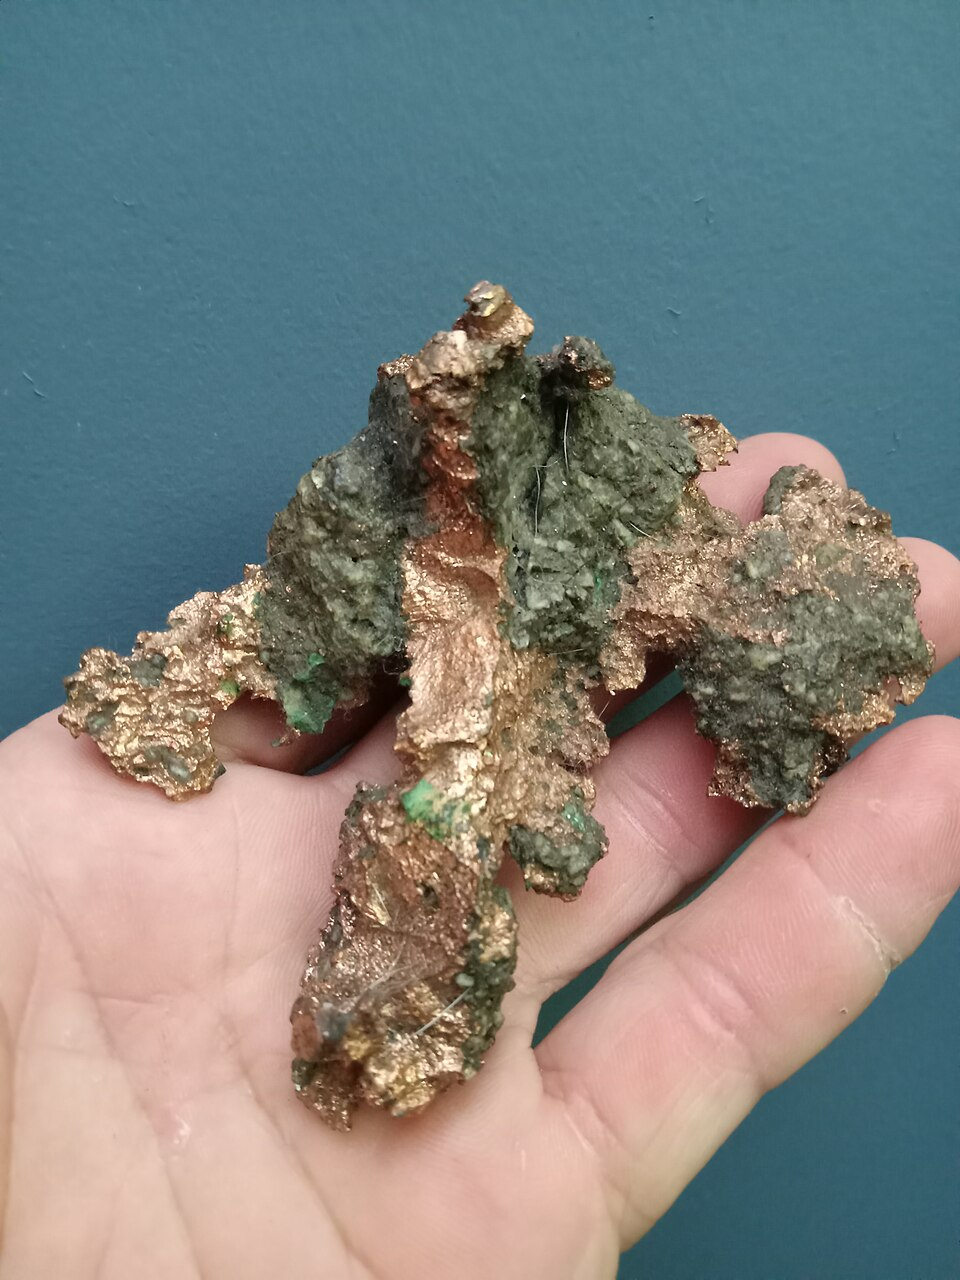
\includegraphics[width=0.36\linewidth]{images/book2/native-copper.jpg}

{\small عيّنة من النحاس الطبيعي. نمت أشكالها المتفرعة على هيئة
بلورات؛ والفلز تحتها فسيفساء من حبيبات مكعبة ممركزة الأوجه.
تصوير: CC0 (ويكيميديا كومنز).}
\end{omfigure}

\section{المواقع البينية}

\begin{definition}[المواقع البينية]\label{def:b1:crystals-metals:site}
\emph{الموقع البيني}\index{موقع بيني} فجوة بين
ذرات \omterm{def:b1:crystals-metals:crystal}{البلورة} يمكن أن تستقر فيها ذرة أصغر. ويقع \emph{الموقع
الرباعي الأوجه}\index{موقع رباعي الأوجه} في مركز رباعي أوجه من أربع
ذرات، و\emph{الموقع الثماني الأوجه}\index{موقع ثماني الأوجه} في مركز
ثماني أوجه من ست. و\emph{قابلية الإسكان}\index{قابلية الإسكان} في
موقع هي نصف قطر أكبر كرة تتسع لها دون أن تُبعد
الذرات المحيطة بعضها عن بعض.
\end{definition}

\begin{proposition}[مواقع بنية المكعب الممركز الأوجه]\label{prop:b1:crystals-metals:sites}
تحوي خلية \omterm{def:b1:crystals-metals:packings}{المكعب الممركز الأوجه} 4 \omterm{def:b1:crystals-metals:site}{مواقع ثمانية الأوجه}، في مركز المكعب وفي
منتصفات أحرفه الاثني عشر، و8 \omterm{def:b1:crystals-metals:site}{مواقع رباعية الأوجه}، في مراكز
المكعبات الصغيرة الثمانية التي طول حرفها $a/2$. ومن أجل ذرات متماسة نصف قطرها $R$،
تكون قابليتا الإسكان
\[
  r_O = (\sqrt2 - 1)R \approx 0.414\,R, \qquad
  r_T = \left(\sqrt{\tfrac32} - 1\right)R \approx 0.225\,R .
\]
\end{proposition}

\begin{proof}
\omterm{def:b1:crystals-metals:site}{المواقع الثمانية الأوجه}: $1 + 12 \times \frac14 = 4$، بقدر عدد الذرات. ويبعد
مركز المكعب $a/2$ عن مراكز الأوجه الستة: $r_O + R = a/2$
مع $a = 2\sqrt2 R$، فيكون $r_O = (\sqrt2 - 1)R$. \omterm{def:b1:crystals-metals:site}{المواقع الرباعية الأوجه}:
يبعد مركز مكعب صغير طول حرفه $a/2$ نصف قطره الرئيسي،
$\frac{a}{2}\cdot\frac{\sqrt3}{2} = \frac{a\sqrt3}{4}$، عن الذرات الأربع
الواقعة على رؤوس متناوبة: $r_T + R = \frac{\sqrt3}{4}\,2\sqrt2\,R =
\sqrt{\tfrac32}\,R$.
\end{proof}

\begin{omfigure}
\tdplotsetmaincoords{60}{100}
\begin{tikzpicture}[tdplot_main_coords, font=\small]
  \pic {omcubeo={3}};
  \node[cellA=3.6mm] at (0,0,0) {};
  \node[cellsite=4mm, draw=omThm, fill=omThm!30] at (0,1.5,0) {};
  \node[cellA=3.6mm] at (0,3,0) {};
  \node[cellsite=4mm, draw=omThm, fill=omThm!30] at (0,0,1.5) {};
  \node[cellA=3.6mm] at (0,1.5,1.5) {};
  \node[cellsite=4mm, draw=omThm, fill=omThm!30] at (0,3,1.5) {};
  \node[cellsite=4mm, draw=omThm, fill=omThm!30] at (1.5,0,0) {};
  \node[cellA=3.6mm] at (0,0,3) {};
  \node[cellA=3.6mm] at (1.5,1.5,0) {};
  \node[cellsite=4mm, draw=omThm, fill=omThm!30] at (0,1.5,3) {};
  \node[cellsite=4mm, draw=omThm, fill=omThm!30] at (1.5,3,0) {};
  \node[cellA=3.6mm] at (0,3,3) {};
  \node[cellA=3.6mm] at (1.5,0,1.5) {};
  \node[cellsite=5mm, draw=omThm, fill=omThm!30] at (1.5,1.5,1.5) {};
  \node[cellA=3.6mm] at (1.5,3,1.5) {};
  \node[cellA=3.6mm] at (3,0,0) {};
  \node[cellsite=4mm, draw=omThm, fill=omThm!30] at (1.5,0,3) {};
  \node[cellsite=4mm, draw=omThm, fill=omThm!30] at (3,1.5,0) {};
  \node[cellA=3.6mm] at (1.5,1.5,3) {};
  \node[cellA=3.6mm] at (3,3,0) {};
  \node[cellsite=4mm, draw=omThm, fill=omThm!30] at (1.5,3,3) {};
  \node[cellsite=4mm, draw=omThm, fill=omThm!30] at (3,0,1.5) {};
  \node[cellA=3.6mm] at (3,1.5,1.5) {};
  \node[cellsite=4mm, draw=omThm, fill=omThm!30] at (3,3,1.5) {};
  \node[cellA=3.6mm] at (3,0,3) {};
  \node[cellsite=4mm, draw=omThm, fill=omThm!30] at (3,1.5,3) {};
  \node[cellA=3.6mm] at (3,3,3) {};
  \node[below] at (1.5,1.5,-1.5) {المواقع الثمانية الأوجه، بالأحمر};
\end{tikzpicture}
\hspace{1.2cm}
\begin{tikzpicture}[tdplot_main_coords, font=\small]
  \pic {omcubeo={3}};
  \node[cellA=3.6mm] at (0,0,0) {};
  \node[cellA=3.6mm] at (0,3,0) {};
  \node[cellA=3.6mm] at (0,1.5,1.5) {};
  \node[cellsite=4mm, fill=omDef!30] at (0.75,0.75,0.75) {};
  \node[cellsite=4mm, fill=omDef!30] at (0.75,2.25,0.75) {};
  \node[cellA=3.6mm] at (0,0,3) {};
  \node[cellA=3.6mm] at (1.5,1.5,0) {};
  \node[cellsite=4mm, fill=omDef!30] at (0.75,0.75,2.25) {};
  \node[cellA=3.6mm] at (0,3,3) {};
  \node[cellA=3.6mm] at (1.5,0,1.5) {};
  \node[cellsite=4mm, fill=omDef!30] at (0.75,2.25,2.25) {};
  \node[cellsite=4mm, fill=omDef!30] at (2.25,0.75,0.75) {};
  \node[cellA=3.6mm] at (1.5,3,1.5) {};
  \node[cellA=3.6mm] at (3,0,0) {};
  \node[cellsite=4mm, fill=omDef!30] at (2.25,2.25,0.75) {};
  \node[cellA=3.6mm] at (1.5,1.5,3) {};
  \node[cellA=3.6mm] at (3,3,0) {};
  \node[cellsite=4mm, fill=omDef!30] at (2.25,0.75,2.25) {};
  \node[cellsite=4mm, fill=omDef!30] at (2.25,2.25,2.25) {};
  \node[cellA=3.6mm] at (3,1.5,1.5) {};
  \node[cellA=3.6mm] at (3,0,3) {};
  \node[cellA=3.6mm] at (3,3,3) {};
  \draw[omDef!70!black, thin] (0,0,0) -- (0.75,0.75,0.75) -- (1.5,1.5,0)
    (0.75,0.75,0.75) -- (1.5,0,1.5) (0.75,0.75,0.75) -- (0,1.5,1.5);
  \node[below] at (1.5,1.5,-1.5) {المواقع الرباعية الأوجه، بالأزرق};
\end{tikzpicture}

{\small \omterm{def:b1:crystals-metals:site}{المواقع البينية} في خلية \omterm{def:b1:crystals-metals:packings}{المكعب الممركز الأوجه}. يمينًا: \omterm{def:b1:crystals-metals:site}{الموقع الثماني الأوجه} في
المركز والمواقع الواقعة في منتصفات الأحرف (تشترك في كل منها أربع خلايا). يسارًا:
\omterm{def:b1:crystals-metals:site}{المواقع الرباعية الأوجه} الثمانية في مراكز أثمان المكعب،
وقد وُصل أحدها بذراته الأربع.}
\end{omfigure}

\section{الرابطة الفلزية والسبائك}

\begin{definition}[الرابطة الفلزية]\label{def:b1:crystals-metals:metallic-bond}
في \emph{الرابطة الفلزية}\index{رابطة فلزية}، تمنح كل ذرة من الفلز
إلكترونات تكافئها \omterm{def:b1:crystals-metals:crystal}{للبلورة} كلها: فالجسم الصلب \omterm{def:b1:crystals-metals:lattice}{شبكة}
من الكاتيونات مغمورة في إلكترونات لا تنتمي إلى ذرة بعينها
وتتحرك فيه بحرية. والرابطة هي التجاذب بين الكاتيونات
وهذه السحابة الإلكترونية المشتركة؛ وهي غير موجّهة.
\end{definition}

\begin{proposition}[خواص الفلزات]\label{prop:b1:crystals-metals:properties}
تفسر \omterm{def:b1:crystals-metals:metallic-bond}{الرابطة الفلزية} خواص الفلزات: فالإلكترونات المتحركة
توصل الكهرباء والحرارة وتعكس الضوء (البريق)؛ ولأن الرابطة
غير موجّهة، تستطيع طبقات الذرات أن تنزلق بعضها على بعض دون
أن تنكسر \omterm{def:b1:crystals-metals:crystal}{البلورة} (المطيلية، وقابلية الطرق)، وأنواع \omterm{def:b1:crystals-metals:packings}{الرصّ المتراصّ}، التي
تجعل عدد الجيران أعظميًا، هي أشيع البنى.
\end{proposition}
\admitted

\begin{definition}[السبائك]\label{def:b1:crystals-metals:alloy}
السبيكة جسم صلب فلزي مكوّن من عدة عناصر. ففي
\emph{السبيكة الاستبدالية}\index{سبيكة استبدالية} تحلّ ذرات
العنصر المضاف محل ذرات المضيف على شبكته؛ وهذا يقتضي
أن يتقارب نصفا القطرين في حدود 15\,\% تقريبًا (النحاس والنيكل، والنحاس
والزنك في النحاس الأصفر). وفي \emph{السبيكة البينية}\index{سبيكة بينية}
تشغل ذرات صغيرة (\ce{H}، \ce{C}، \ce{N}، \ce{B}) \omterm{def:b1:crystals-metals:site}{مواقع بينية} في
المضيف (الكربون في الفولاذ).
\end{definition}

\begin{definition}[التآصل]\label{def:b1:crystals-metals:allotropy}
البنى البلورية المختلفة للعنصر نفسه هي
\emph{متآصلاته}\index{متآصل}. فالحديد \omterm{def:b1:crystals-metals:packings}{مكعب ممركز الجسم} (الحديد $\alpha$) في درجة حرارة
الغرفة؛ وقد قيس مكعبًا ممركز الأوجه (الحديد $\gamma$) من \qty{1189}{K}
إلى \qty{1661}{K}، ثم مكعبًا ممركز الجسم مرة أخرى (الحديد $\delta$) عند \qty{1662}{K}، وحتى
نقطة انصهاره. ويوجد الكربون ألماسًا وغرافيتًا
(\cref{ch:b1:crystals-ionic-covalent}).
% ledger: lat:Fe-alpha, lat:Fe-gamma-1189, lat:Fe-gamma-1661,
% lat:Fe-delta-1662
\end{definition}

\begin{example}[الفولاذ]\label{ex:b1:crystals-metals:steel}
الكربون، الذي نصف قطره التساهمي \qty{77}{pm} (نصف المسافة \ce{C-C} في
الألماس)، أكبر من أن تتسع له مواقع الحديد دون تشويه، لكنه
أقل بكثير تجاوزًا في الحديد $\gamma$، الذي مواقعه الثمانية الأوجه هي الأكبر. ويُصنع
الفولاذ بإذابة الكربون في الحديد $\gamma$ الساخن؛ فإذا سُقي انحبس
الكربون بينما يعود الحديد إلى بنية ممركزة الجسم، فيشوّهها،
\omterm{def:b1:crystals-metals:crystal}{والبلورة} المشوّهة صلدة.
% ledger: lat:C-diamond (r = a sqrt3 / 8 = 77.2 pm)
\end{example}

\begin{remark}[تحولات الحديد]\label{rem:b1:crystals-metals:iron-T}
درجات الحرارة الواردة في \cref{def:b1:crystals-metals:allotropy} هي درجات
الحديد النقي تحت الضغط الجوي؛ والكربون المذاب يخفض
درجة الحرارة التي يتكوّن عندها الحديد $\gamma$، وهذا ما يجعل الفولاذ قابلًا للتشكيل.
وتُدرس مخططات أطوار السبائك في مجلد السنة الثانية.
\end{remark}

\section{تمارين}

\begin{exercise}[$\star$]\label{exo:b1:crystals-metals:1}
عُدّ ذرات خلية مكعبة بسيطة (ذرات على الرؤوس فقط)، وخلية
مكعبة ممركزة الجسم، وخلية مكعبة ممركزة الأوجه، وأعطِ \omterm{def:b1:crystals-metals:coordination}{عدد التناسق} في كل منها.
\end{exercise}

\begin{exercise}[$\star$]\label{exo:b1:crystals-metals:2}
بيّن أن \omterm{def:b1:crystals-metals:compactness}{اكتناز} البنية المكعبة البسيطة (الذرات متماسة
على امتداد الحرف) هو $\pi/6$، وقارنه \omterm{def:b1:crystals-metals:compactness}{باكتناز} البنيتين الممركزة الأوجه والممركزة الجسم.
\end{exercise}

\begin{exercise}[$\star$]\label{exo:b1:crystals-metals:3}
الألومنيوم \omterm{def:b1:crystals-metals:packings}{مكعب ممركز الأوجه} مع $a = \qty{405.0}{pm}$. احسب نصف قطره الذري
وكتلته الحجمية ($M = \qty{26.98}{g/mol}$).
% ledger: lat:Al, aw:Al
\end{exercise}

\begin{exercise}[$\star$]\label{exo:b1:crystals-metals:4}
الصوديوم \omterm{def:b1:crystals-metals:packings}{مكعب ممركز الجسم} مع $a = \qty{429.1}{pm}$. احسب نصف قطره الذري
وكتلته الحجمية ($M = \qty{22.99}{g/mol}$)، وقارن بالقيمة المقيسة
\qty{0.97}{g/cm^3}.
% ledger: lat:Na, rho:Na, aw:Na
\end{exercise}

\begin{exercise}[$\star\star$]\label{exo:b1:crystals-metals:5}
الفضة مكعبة ممركزة الأوجه وكتلتها الحجمية \qty{10.50}{g/cm^3}
($M = \qty{107.87}{g/mol}$). احسب وسيط \omterm{def:b1:crystals-metals:lattice}{الشبكة} ونصف القطر
الذري.
% ledger: rho:Ag, aw:Ag
\end{exercise}

\begin{exercise}[$\star\star$]\label{exo:b1:crystals-metals:6}
بيّن أن $c/a = \sqrt{8/3}$ في بنية سداسية متراصّة من كرات متماسة.
للمغنيسيوم $a = \qty{320.9}{pm}$، $c = \qty{521.0}{pm}$. احسب $c/a$
والكتلة الحجمية للمغنيسيوم ($M = \qty{24.31}{g/mol}$).
% ledger: lat:Mg.a, lat:Mg.c, aw:Mg
\end{exercise}

\begin{exercise}[$\star\star$]\label{exo:b1:crystals-metals:7}
في خلية مكعبة ممركزة الأوجه طول حرفها $a$، أعطِ إحداثيات الذرات الأربع التي
تعود إلى الخلية، \omterm{def:b1:crystals-metals:site}{والمواقع الثمانية الأوجه} الأربعة \omterm{def:b1:crystals-metals:site}{والمواقع الرباعية الأوجه}
الثمانية. كم موقعًا من كل نوع لكل ذرة؟
\end{exercise}

\begin{exercise}[$\star\star$]\label{exo:b1:crystals-metals:8}
النحاس والنيكل كلاهما \omterm{def:b1:crystals-metals:packings}{مكعب ممركز الأوجه}، مع $a = \qty{361.5}{pm}$
و$a = \qty{352.4}{pm}$. احسب نصفي قطريهما الذريين. إنهما يكوّنان
\omterm{def:b1:crystals-metals:alloy}{سبيكة استبدالية} بكل النسب: فسّر. وأي نوع من السبائك يستطيع
الهيدروجين، وهو ذرة صغيرة جدًا، أن يكوّنه مع فلز؟
% ledger: lat:Cu, lat:Ni
\end{exercise}

\begin{exercise}[$\star\star$]\label{exo:b1:crystals-metals:9}
التنغستن \omterm{def:b1:crystals-metals:packings}{مكعب ممركز الجسم} مع $a = \qty{316.5}{pm}$. احسب نصف قطره،
وكتلته الحجمية ($M = \qty{183.84}{g/mol}$) وعدد الذرات في
\qty{1}{cm^3}.
% ledger: lat:W, aw:W
\end{exercise}

\begin{exercise}[$\star\star\star$]\label{exo:b1:crystals-metals:10}
في بنية \omterm{def:b1:crystals-metals:packings}{المكعب الممركز الجسم} يقع \omterm{def:b1:crystals-metals:site}{موقع ثماني الأوجه} في مركز كل وجه
(وفي منتصف كل حرف)، ويقع \omterm{def:b1:crystals-metals:site}{موقع رباعي الأوجه} عند
$(\frac{a}{2}, \frac{a}{4}, 0)$ على كل وجه. بيّن أن
قابليتي إسكانهما $r_O = \frac{2 - \sqrt3}{4}\,a$
و$r_T = \frac{\sqrt5 - \sqrt3}{4}\,a$، وعبّر عنهما كسرين من
$R$. أي الموقعين أكبر؟
\end{exercise}

\begin{exercise}[$\star\star\star$]\label{exo:b1:crystals-metals:11}
يتبلور فلز بعدد $Z$ من الذرات في كل خلية مكعبة طول حرفها $a$. بيّن أن
\omterm{def:b1:crystals-metals:compactness}{الاكتناز} يمكن أن يُكتب $C = \frac{4\pi R^3 Z}{3a^3}$، ثم أن
$C = \frac{\pi\rho N_A}{6M}\,(2R)^3$. وطبّق على النحاس ($R = \qty{127.8}{pm}$،
$\rho = \qty{8.93}{g/cm^3}$) للتحقق من القيمة $0.74$.
\end{exercise}

\begin{exercise}[$\star\star\star$]\label{exo:b1:crystals-metals:12}
الذهب \omterm{def:b1:crystals-metals:packings}{مكعب ممركز الأوجه} مع $a = \qty{407.8}{pm}$ والفضة مكعبة ممركزة الأوجه مع
$a = \qty{408.6}{pm}$. والذهب والفضة يمتزجان بكل النسب. قدّر
وسيط \omterm{def:b1:crystals-metals:lattice}{الشبكة} لسبيكة فيها 50\,\% من ذرات كل منهما (افترض
المتوسط) وكتلتها الحجمية ($M(\ce{Au}) = \qty{196.97}{g/mol}$،
$M(\ce{Ag}) = \qty{107.87}{g/mol}$).
% ledger: lat:Au, lat:Ag, aw:Au, aw:Ag
\end{exercise}

\section{مسألة: لماذا يمسك الفولاذ الكربون}

\begin{problem}[{مسألة نهاية الأسبوع --- الحديد تحت تحوله وفوقه
قرب 1190\,K، والفجوات بين ذراته، والحيز الذي تتركه
للكربون}]
\label{pb:b1:crystals-metals:1}
معطيات: $M(\ce{Fe}) = \qty{55.845}{g/mol}$، $M(\ce{C}) = \qty{12.011}{g/mol}$،
$N_A = \qty{6.022e23}{mol^{-1}}$. في درجة حرارة الغرفة يكون الحديد $\alpha$ مكعبًا ممركز الجسم
مع $a = \qty{286.65}{pm}$. وعند \qty{1189}{K}، فوق التحول مباشرة،
يُقاس الحديد $\alpha$ (الذي لا يزال موجودًا تحت التحول)
مع $a = \qty{289.8}{pm}$ والحديد $\gamma$، \omterm{def:b1:crystals-metals:packings}{المكعب الممركز الأوجه}، مع $a = \qty{363.9}{pm}$.
والألماس مكعب مع $a = \qty{356.68}{pm}$، وكل كربون فيه يمسّ أربعة
أخرى على ربع القطر الرئيسي.
% ledger: lat:Fe-alpha, lat:Fe-alpha-1189, lat:Fe-gamma-1189,
% lat:C-diamond, aw:Fe, aw:C, const:NA

\medskip
\noindent\textbf{الجزء الأول --- الحديد $\alpha$ في درجة حرارة الغرفة.}
\begin{enumerate}
  \item كم ذرة تعود إلى خلية مكعبة ممركزة الجسم؟ وما \omterm{def:b1:crystals-metals:coordination}{عدد
        التناسق}؟
  \item على امتداد أي خط تتماس الذرات؟ احسب نصف قطر
        ذرة الحديد.
  \item احسب الكتلة الحجمية للحديد $\alpha$.
  \item كم ذرة حديد في \qty{1}{cm^3} من الحديد $\alpha$؟
  \item احسب \omterm{def:b1:crystals-metals:compactness}{اكتناز} بنية \omterm{def:b1:crystals-metals:packings}{المكعب الممركز الجسم}.
  \item قارن بالكتلة الحجمية المقيسة، \qty{7.87}{g/cm^3}.
% ledger: rho:Fe
\end{enumerate}

\medskip
\noindent\textbf{الجزء الثاني --- عبور التحول.}
\begin{enumerate}[resume]
  \item احسب نصف قطر ذرة الحديد في الحديد $\alpha$ وفي
        الحديد $\gamma$ عند \qty{1189}{K}.
  \item احسب الحجم لكل ذرة في كل طور.
  \item أي الطورين أكثف؟ احسب الكتلتين الحجميتين.
  \item بأي نسبة مئوية يتغير حجم قضيب حين ينتقل
        من $\alpha$ إلى $\gamma$ بالتسخين؟
  \item هل تتسق النتيجة مع اكتنازي
        البنيتين؟
\end{enumerate}

\medskip
\noindent\textbf{الجزء الثالث --- الفجوات في الحديد $\alpha$.}
\begin{enumerate}[resume]
  \item انطلاقًا من بنية الألماس، احسب \omterm{def:b1:periodicity:radius}{نصف القطر التساهمي} للكربون.
  \item في الحديد $\alpha$ \omterm{def:b1:crystals-metals:packings}{المكعب الممركز الجسم} عند \qty{1189}{K}، احسب \omterm{def:b1:crystals-metals:site}{قابلية الإسكان}
        في \omterm{def:b1:crystals-metals:site}{موقع ثماني الأوجه}، $r_O = \frac{2 - \sqrt3}{4}\,a$.
  \item احسب \omterm{def:b1:crystals-metals:site}{قابلية الإسكان} في \omterm{def:b1:crystals-metals:site}{موقع رباعي الأوجه}، $r_T = \frac{\sqrt5 -
        \sqrt3}{4}\,a$.
  \item قارن بنصف قطر الكربون. ماذا يجب أن يحدث
        \omterm{def:b1:crystals-metals:lattice}{للشبكة} حول ذرة كربون؟
  \item فسّر لماذا لا يذوب الكربون إلا بكميات ضئيلة في
        الحديد $\alpha$.
\end{enumerate}

\medskip
\noindent\textbf{الجزء الرابع --- الفجوات في الحديد $\gamma$.}
\begin{enumerate}[resume]
  \item كم موقعًا ثماني الأوجه تحوي خلية مكعبة ممركزة الأوجه من الحديد $\gamma$،
        لكل ذرة حديد؟
  \item احسب \omterm{def:b1:crystals-metals:site}{قابلية الإسكان} في \omterm{def:b1:crystals-metals:site}{موقع رباعي الأوجه} من الحديد $\gamma$.
  \item لو مُلئت كل \omterm{def:b1:crystals-metals:site}{المواقع الثمانية الأوجه} بالكربون، فما
        صيغة الجسم الصلب والكسر الكتلي للكربون؟
  \item لو مُلئ \omterm{def:b1:crystals-metals:site}{موقع ثماني الأوجه} واحد من كل عشرة، فكم يكون الكسر
        الكتلي للكربون؟
  \item فسّر لماذا يُصنع الفولاذ بإذابة الكربون في الحديد الساخن.
  \item احسب نصف قطر أكبر كرة تتسع لها
        \omterm{def:b1:crystals-metals:site}{المواقع الثمانية الأوجه} في الحديد $\gamma$.
\end{enumerate}
\end{problem}
